\subsection*{Introduction}

How did species come to live where they're found today?
To answer this, we can leverage phylogenetic, molecular, and geographical information to model species distributions as the outcome of biogeographic processes.
How to best model these processes requires special consideration, such as how ranges are inherited following speciation events, how geological events might influence dispersal rates, and what factors affect rates of dispersal and extirpation.
A major technical challenge of modeling range evolution is how to translate these natural processes into stochastic processes that remain tractable for inference.
This tutorial provides a brief background in some of these models, then describes how to perform Bayesian inference of historical biogeography using \RevBayes.

\section{Overview of the Dispersal-Extinction-Cladogenesis model}

\subsection*{Discrete range characters}

The Dispersal-Extinction-Cladogenesis (DEC) models range evolution as a discrete-valued process \citep{Ree2005, Ree2008}.
DEC interprets taxon ranges as presence-absence data, that is, where a species is observed or not observed across multiple discrete areas.
For example, say there are three areas, A, B, and C.
If a species is present in areas A and C, then its range equals AC, which can also be encoded into the length-3 bit vector, 101.
Bit vectors may also be transformed into (decimal) integers, \EG the binary number 101 equals the decimal number 5.

%\begin{center}
\begin{table}[!ht]
\scriptsize
\centering
\begin{tabular}{lrcc}
Range & Bits & Size & State \\ \hline
$\emptyset$ & 000 & 0 & 0 \\
          A & 100 & 1 & 1 \\
          B & 010 & 1 & 2 \\
          C & 001 & 1 & 3 \\
         AB & 110 & 2 & 4 \\
         AC & 101 & 2 & 5 \\
         BC & 011 & 2 & 6 \\
        ABC & 111 & 3 & 7 \\
\end{tabular}
\caption{Example of discrete range representations for an analysis with areas A, B, and C.}
\end{table}
%\end{center}

Decimal representation is rarely used in discussion, but it is useful to keep in mind when considering the total number of possible ranges for a species and when processing output.
Note, \RevBayes assigns integers to ranges in order according to size.

\subsection*{Anagenetic range evolution}


Anagenesis refers to range evolution that occurs between speciation events within lineages.
Because DEC uses discrete-valued ranges, anagenesis is modeled using a continuous-time Markov chain.
This, in turn, allows us to compute transition probability of a character changing from $i$ to $j$ in time $t$ through matrix exponentiation
\[
\mathbf{P}_{ij}(t) = \left[ \exp \left\lbrace \mathbf{Q}t \right\rbrace \right]_{ij},
\]
where $\textbf{Q}$ is the instantaneous rate matrix defining the rates of change between all pairs of characters, and $\textbf{P}$ is the transition probability rate matrix.
The indices $i$ and $j$ represent different ranges, each of which is encoded as the set of areas occupied by the species.
The probability has integrated over all possible scenarios of character transitions that could occur during $t$ so long as the chain begins in state $i$ and ends in state $j$.

We can then encode ${\bf Q}$ to reflect the allowable classes of range evolution events with biologically meaningful parameters.
We'll take a simple model of range expansion (e.g. $BC \rightarrow ABC$) and range contraction (e.g. $BC \rightarrow C$).
Range expansion may also be referred to as dispersal or area gain and range contraction as extirpation, (local) extinction, or area loss.
The rates in the transition matrix for three areas might appear as

\[
\textbf{Q} = 
	\begin{array}{c|cccccccc}
		& \emptyset & A & B & C & AB & AC & BC & ABC \\
		\hline
		\emptyset 	& - 	& 0 	& 0 	& 0 		& 0			& 0 		& 0 		& 0 \\
		A 			& e_A 	& - 	& 0 	& 0 		& d_{AB}	& d_{AC} 	& 0 		& 0 \\
		B 			& e_B 	& 0 	& - 	& 0 		& d_{BA}	& 0 		& d_{BC} 	& 0 \\
		C 			& e_C 	& 0 	& 0 	& - 		& 0 		& d_{CA} 	& d_{CB} 	& 0 \\
		AB 			& 0 	& e_A 	& e_B 	& 0 		& -			& 0 		& 0 		& d_{AC} + d_{BC} \\
		AC 			& 0 	& e_C 	& 0 	& e_A 		& 0			& - 		& 0 		& d_{AB} + d_{CB} \\
		BC 			& 0 	& 0 	& e_C 	& e_B 		& 0			& 0 		& - 		& d_{BA} + d_{CA} \\
		ABC 		& 0 	& 0 	& 0 	& 0 		& e_C 		& e_B 		& e_A 		& - \\								
	\end{array}
\]

where $e = ( e_A, e_B, e_C )$ are the (local) extinction rates per area, and $d = ( d_{AB}, d_{AC}, d_{BC}, d_{BA}, d_{CA}, d_{CB})$ are the dispersal rates between areas.
Notice that the sum of rates leaving the null range ($\emptyset$) is zero, meaning any lineage that loses all areas in its range remains that way permanently.

To build our intuition, let's build a DEC rate matrix.
Assume you have three areas

\begin{snugshade}
\begin{lstlisting}
n_areas <- 3
\end{lstlisting}
\end{snugshade}

First, create a matrix of dispersal rates between area pairs, with rates $d_{AB} = d_{AC} = \ldots = d_{CB} = 1$

\begin{snugshade}
\begin{lstlisting}
for (i in 1:n_areas) {
    for (j in 1:n_areas) {
        dr[i][j] <- abs(1)
    }
}
\end{lstlisting}
\end{snugshade}

Next, let's create the extirpation rates with values $e_A=e_B=e_C=1$

\begin{snugshade}
\begin{lstlisting}
for (i in 1:n_areas) {
    for (j in 1:n_areas) {
        er[i][j] <- abs(0)
    }
    er[i][i] <- abs(1) 
}
\end{lstlisting}
\end{snugshade}

When the extirpation rate matrix is a diagonal matrix (i.e. all non-diagonal entries are zero), extirpation rates are mutually independent as in \citep{Ree2005}.
More complex models that penalize widespread ranges that span disconnected areas are explored in later sections.

To continue, create the DEC rate matrix from the dispersal rates ({\tt dr}) and extirpation rates ({\tt er}).

\begin{snugshade}
\begin{lstlisting}
Q_DEC := fnDECRateMatrix(dispersalRates=dr, extirpationRates=er)
Q_DEC
[ [ 0.0000, 0.0000, 0.0000, 0.0000, 0.0000, 0.0000, 0.0000, 0.0000 ] ,
     1.0000, -3.0000, 0.0000, 0.0000, 1.0000, 1.0000, 0.0000, 0.0000 ] ,
     1.0000, 0.0000, -3.0000, 0.0000, 1.0000, 0.0000, 1.0000, 0.0000 ] ,
     1.0000, 0.0000, 0.0000, -3.0000, 0.0000, 1.0000, 1.0000, 0.0000 ] ,
     0.0000, 1.0000, 1.0000, 0.0000, -4.0000, 0.0000, 0.0000, 2.0000 ] ,
     0.0000, 1.0000, 0.0000, 1.0000, 0.0000, -4.0000, 0.0000, 2.0000 ] ,
     0.0000, 0.0000, 1.0000, 1.0000, 0.0000, 0.0000, -4.0000, 2.0000 ] ,
     0.0000, 0.0000, 0.0000, 0.0000, 1.0000, 1.0000, 1.0000, -3.0000 ] ]
\end{lstlisting}
\end{snugshade}

Compute the anagenetic transition probabilities for a branch of length {\tt 0.2}.

\begin{snugshade}
\begin{lstlisting}
tp_DEC <- Q_DEC.getTransitionProbabilities(rate=0.2)
tp_DEC
[ [ 1.000, 0.000, 0.000, 0.000, 0.000, 0.000, 0.000, 0.000],
  [ 0.000, 0.673, 0.013, 0.013, 0.123, 0.123, 0.005, 0.050],
  [ 0.000, 0.013, 0.673, 0.013, 0.123, 0.005, 0.123, 0.050],
  [ 0.000, 0.013, 0.013, 0.673, 0.005, 0.123, 0.123, 0.050],
  [ 0.000, 0.107, 0.107, 0.004, 0.502, 0.031, 0.031, 0.218],
  [ 0.000, 0.107, 0.004, 0.107, 0.031, 0.502, 0.031, 0.218],
  [ 0.000, 0.004, 0.107, 0.107, 0.031, 0.031, 0.502, 0.218],
  [ 0.000, 0.021, 0.021, 0.021, 0.107, 0.107, 0.107, 0.616]]
\end{lstlisting}
\end{snugshade}

Notice how the structure of the rate matrix is reflected in the transition probability matrix.
For example, ranges that are separated by multiple dispersal and extirpation events are the most improbable: transitioning from going from A to BC takes a minimum of three events and has probability 0.005.

Also note that the probability of entering or leaving the null range is zero.
By default, the \RevBayes conditions the anagenetic range evolution process on never entering the null range when computing the transition probabilities ({\tt nullRange=CondSurv}).
This allows the model to both simulate and infer using the same transition probabilities.
\citet{Massana2015} first noted that the null range results in abnormal extirpation rate and range size estimates.
Their proposed solution to eliminate the null range from the state space is enabled with the {\tt nullRange=Exclude} setting. 
The {\tt nullRange=Include} setting provides no special handling of the null range, and produces the raw probabilities of \citet{Ree2005}.

\subsection*{Cladogenetic range evolution}

The cladogenetic component of the DEC model describes evolutionary change accompanying speciation events.
In the context of range evolution, daughter species do not necessarily inherit their ancestral range in an identical manner.
For each internal node in the reconstructed tree, one of several cladogenetic events can occur, some of which are described below.

Beginning with the simplest case first, suppose the range of a species is $A$ the moment before speciation occurs at an internal phylogenetic node.
Since the species range is size one, both daughter lineages necessarily inherit the ancestral species range ($A$).
In DEC parlance, this is called a narrow sympatry event.
Now, suppose the ancestral range is $ABC$.
Under subset sympatry, one lineage identically inherits the ancestral species range, $ABC$, while the other lineage inherits only a single area, i.e. only $A$ or $B$ or $C$.
For widspread sympatric cladogenesis, both lineages inherit the ancestral range, $ABC$.
Under allopatric cladogenesis, the ancestral range is split evenly among daughter lineages, e.g. one lineage may inherit $AB$ and the other inherits $C$.
Finally, supposing the ancestral range is $A$, jump dispersal cladogenesis results in one daughter lineage inheriting the ancestral range $A$, and the other daughter lineage inheriting a previously uninhabited area, $B$ or $C$.
See \citet{Matzke2012} for an excellent overview of the cladogenetic state transitions described in the literature.

Make the cladogenetic probability event matrix

\begin{snugshade}
\begin{lstlisting}
clado_event_types = [ "s", "a" ]
clado_event_probs <- simplex( 1, 1 )
P_DEC := fnDECCladoProbs(eventProbs=clado_event_probs,
                         eventTypes=clado_event_types,
                         numCharacters=n_areas)
\end{lstlisting}
\end{snugshade}

{\tt clado\_event\_types} defines what cladogenetic event types are used.
{\tt "a"} and {\tt "s"} indicate allopatry and subset sympatry, as described in \citep{Ree2005}.
Other cladogenetic events include jump dispersal \citep[{\tt "j"};][]{Matzke2012} and full sympatry \citep[{\tt "f"};][]{Landis2013a}.
The cladogenetic event probability matrix will assume that {\tt eventProbs} and {\tt eventTypes} share the same order.

Print the cladogenetic transition probabilities

\begin{snugshade}
\begin{lstlisting}
P_DEC
   [
     ( 1 -> 1, 1 ) = 1.0000,
     ( 2 -> 2, 2 ) = 1.0000,
     ( 3 -> 3, 3 ) = 1.0000,
     ...
     ( 7 -> 7, 1 ) = 0.0833,
     ( 7 -> 7, 2 ) = 0.0833,
     ( 7 -> 7, 3 ) = 0.0833
   ]
\end{lstlisting}
\end{snugshade}

The cladogenetic probability matrix becomes very sparse for large numbers of areas, so only non-zero values are shown.
Each row reports a triplet of states---the ancestral state and the two daughter states---with the probability associated with that event.
Since these are proper probabilities, the sum of probabilities for a given ancestral state over all possible cladogenetic outcomes equals one.

\subsection*{Things to consider}

The probabilities of anagenetic change along lineages must account for all combinations of starting states and ending states.
For 3 areas, there are 8 states, and thus $8 \times 8 = 64$ probability terms for pairs of states.
For cladogenetic change, we need transition probabilities for all combinations of states before cladogenesis, after cladogenesis for the left lineage, and after cladogenesis for the right lineage.
Like above, for three areas, there are 8 states, and $8 \times 8 \times 8 = 512$ cladogenetic probability terms.

Of course, this model can be specified for more than three areas.
Let's consider what happens to the size of \textbf{Q} when the number of areas, $N$, becomes large.
For three areas, \textbf{Q} is size $8 \times 8$.
For ten areas, \textbf{Q} is size $2^{10} \times 2^{10} = 1024 \times 1024$, which approaches the largest size matrices that can be exponentiated in a practical amount of time.
For twenty areas, \textbf{Q} is size $2^{20} \times 2^{20} \approx 10^6 \times 10^6$ and exponentiation is not viable.
Thus, selecting the discrete areas for a DEC analysis should be done with regard to what one hopes to learn through the analysis itself.




%Methods to permit are available in \RevBayes, but require complicated inference algorithms and 
%\citep{Landis13}

%The DEC model ignores speciation events hidden by extinction or incomplete taxon sampling.
%The probability of cladogenesis and local extinction events would ideally be linked to a birth-death process, as it is in the GeoSSE model \citep{Goldberg2011}.
%Unfortunately, since the numerical method for SSE models scale poorly, and DEC models remain the only option when the geography has more than two or three areas.
%For more than ten areas, data augmentation may be used to infer ancestral ranges, as described in Section \ref{sec:bayarea}.

\subsection*{Some questions}

{\bf \framebox{?} For the three-area DEC rate matrix above, what is the rate of leaving state AC in terms of dispersal and extinction parameters?}

{\bf \framebox{?} What series of transition events might explain a lineage evolving from range $ABC$ to range $A$? From range $AB$ to range $C$?}

{ \bf \framebox{?} Imagine a DEC rate matrix with four areas, $ABCD$. What would be the dispersal rate for $Q_{BC,BCD}$? How many states does a DEC rate matrix with four areas have? What is the relationship between the number of areas and the number of states under the DEC model? }

{\bf \framebox{?} Given the state is $AB$ before cladogenesis, and allowing subset sympatry, widespread sympatry, and allopatry, what are the 7 possible states in the daughter lineages after cladogenesis?}

{\bf \framebox{?} For three areas, there are three narrow, four widespread, 18 subset sympatric events and 12 allopatric cladogenesis events. What proportion of terms in the cladogenesis matrix are zero?}

\subsection*{Recommended tutorials}

The {\bf Historical Biogeography} tutorial will assume the reader has completed the following \RevBayes tutorials

\begin{itemize}
\item {\bf \Rev Basics}
\item {\bf Molecular Models of Character Evolution}
\item {\bf Running and Diagnosing an MCMC Analysis}
\item {\bf Divergence Time Estimation and Node Calibrations}
\end{itemize}

%\begin{figure}[H]
%\centering
%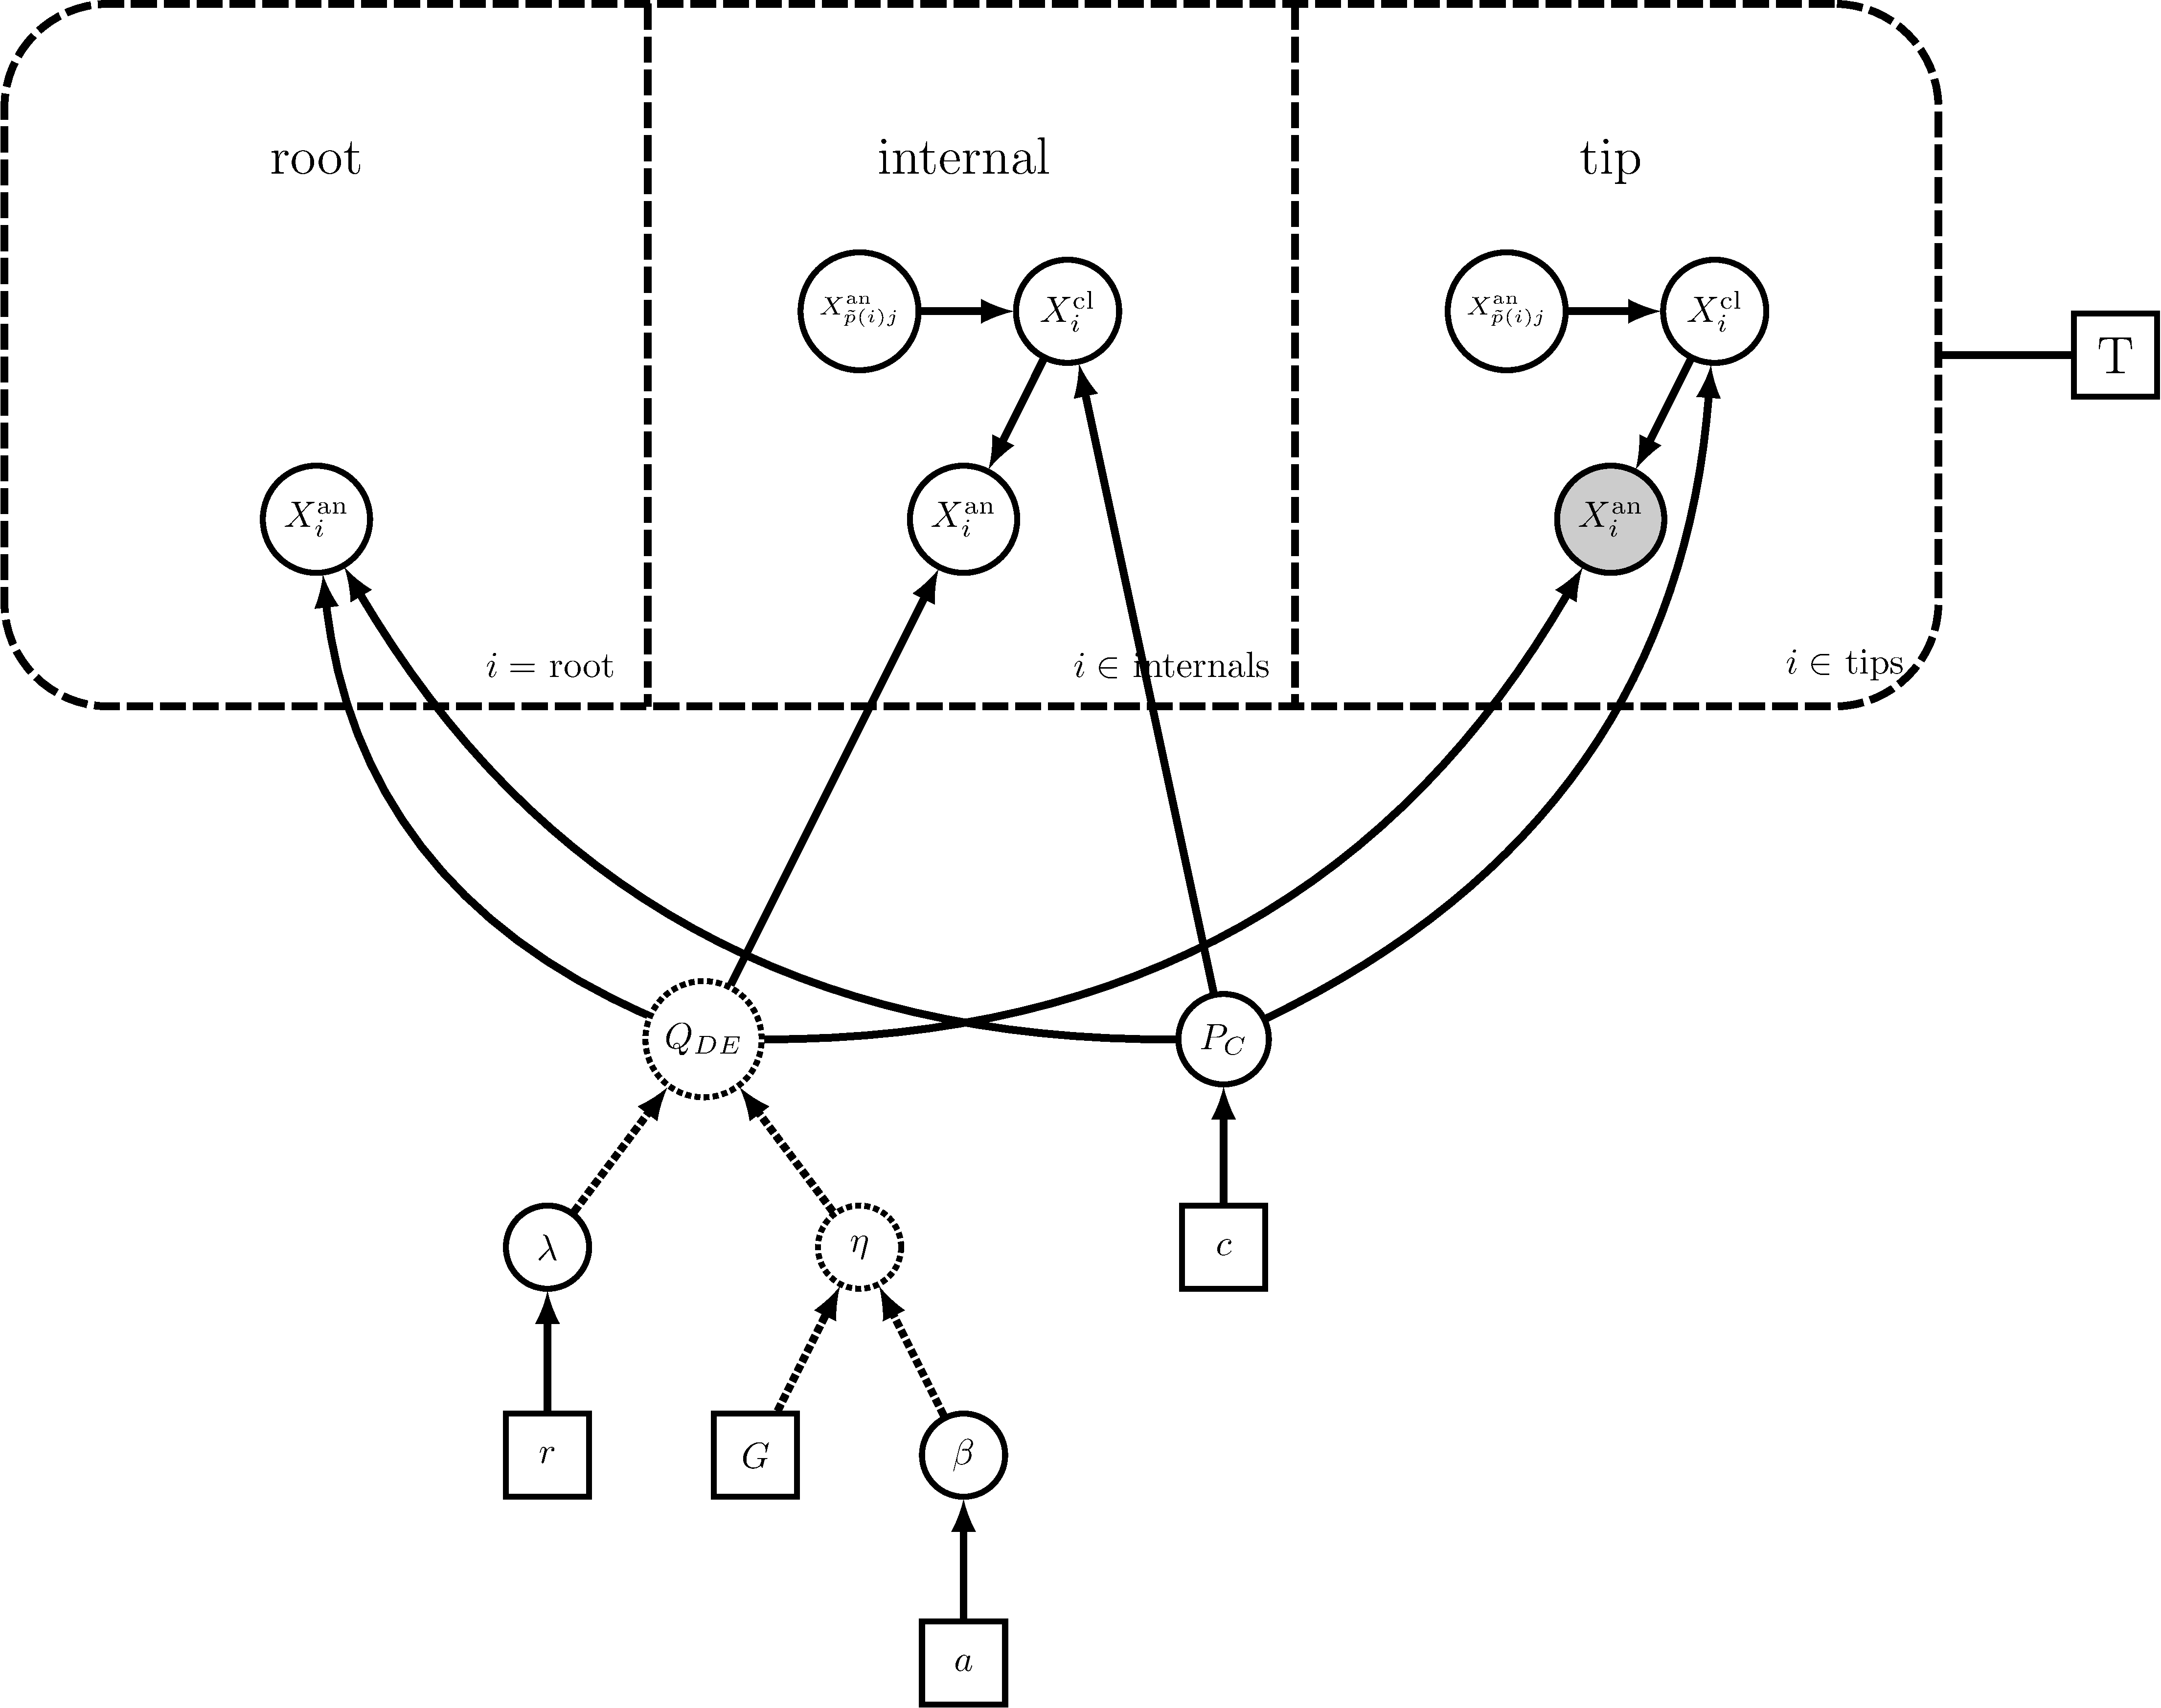
\includegraphics[width=5in]{figures/bg_dec_dag}
%\caption{Graphical model of DEC. The tree plate's topology is fixed by $T$, where each internal node has both an anagenetic and cladogenetic random variable ($X_i^{\text{an}}$ and $X_i^{\text{cl}}$, resp.) that represents an ancestral species before and after it speciated. anagenetic change is modeled by a continuous time Markov process, where $Q_{DE}$ is the instantaneous rate matrix of area gain and loss, as parameterized by $\lambda$. The geographic distance rate modifier function, $\eta$, takes in the geographical distances and strata as $G$, and the distance power parameter, $\beta$. cladogenetic change is modeled by $P_C$, a Dirichlet-distributed simplex with a flat prior.}
%\end{figure}


\newpage
